\documentclass[../../main.tex]{subfiles}
\begin{document}
% As stated in section \ref{sec:ProblemDescription}, the main goal of the project has been to apply knowledge of embedded C and VHDL programming to interface motor encoders in a pan-tilt system, and implement a framework for a discrete controller which allows the robotic system to be manipulated to given positions. Using knowledge gained from the concurrent control systems course, different controller designs and design methods should be assessed, in an attempt to meet the overall system specifications presented in table \ref{tab:performanceSpec}. Simulation results should be compared to results obtained from testing the physical system.

During the project, choices have been made with regards to design of controllers and implementation on the given devices. Some of these choices, both due to inexperience in the disciplines and due to initial project conditions, have proved to be inadequate towards meeting the system response requirements stated by the project group in section \ref{sec:Requirements}.

\subsection{Evaluating Performance}

Ultimately, it must be addressed, that looking at table \ref{tab:controller_data} the specifications initially determined have not been met. In this regard, it must be acknowledged that in fact none of the simulations meet all the specifications either. In hindsight these specifications, especially the one about settling time, have probably been slightly unrealistic from the beginning. Over all it has been possible to achieve performances which are not too dissimilar from those that were found in simulation. It is likely that manually tuning the parameters of the controllers, based on the values presented in this report, could improve the performance. Had more time been available, this would have been interesting to study further. After all, one of the main advantages of the PID-controller is the fact that it is fairly simple to tune. 

Initially, it was expected that the cascaded controller design would yield better results compared to a single controller, at least when implemented, since it theoretically offers better rejection towards noise. With the chosen designs however, the cascaded controllers actually performed worse than the single controller designs in both simulations and implementation. In simulation, this is likely because the velocity controllers should have been designed to meet a faster response. Due to the fact that the control signals on the physical setup is limited to \SI{\pm 12}{\volt}, the controllers were designed in a way that attempted to minimise how much the controls signal saturates. At the same time, the design and tuning of the cascaded controller also becomes more complex, since there are more zeros and pole to consider, and more parameters to tune. 
It was also found that the cascaded controller which relied purely on the mathematical model of the system performed drastically worse than the one which made use of the Ziegler-Nichols tuning method. This is not unexpected, since it is acknowledged that several imperfections in the mathematical model of the motors exist. Therefore a heuristic approach such as the Ziegler-Nichols is likely to yield equally good or better results. That being said, from figure \ref{fig:StepTiltPos}, \ref{fig:StepVelZN} and \ref{fig:Cascade_ZN_tilt} it can be seen that in these cases, the response from the physical system is actually quite close the simulated response for the tilt motor. This indicates that the mathematical model of the tilt motor is in fact pretty decent. The big deviations which are seen in figure \ref{fig:StepVelModel} and \ref{fig:cascade_model_tilt} are likely caused by another issue which is discussed later in section \ref{subsec:}. Figure \ref{fig:StepPanPos} and \ref{fig:cascade_ZN_pan} shows that a lot more deviation is found for the model of the pan motor. This makes sense since the parameters which are found experimentally in section \ref{subsec:motorParameters} are based solely on the tilt motor. If disassembling the pan-tilt system was allowed, it would be interesting to perform similar tests to determine the parameters of the pan motor. From looking at the two figures it also appears that the pan motor generally has a slower response than the model predicts, which among other things could indicate that the estimation of the inertia of the pan motor is too low. This is very likely, as the simplifications, introduced in section \ref{subsec:motorParameters}, will yield a slightly lower result for the inertia especially for the pan motor.  Looking at figure \ref{fig:cascade_ZN_pan} it can be argued that the response from the physical system is in fact more desirable than the simulated response.



% non linear relation between duty cycle and voltage.

% why does the tilt position controller based on model do the best? - something about the best model representation. It seems like the actual pan motor has more inertia than what is modeled. The cascade seems to be worse. Why? because of the poor velocity control.
%discuss the fact that the requirements are not met. Could we have met them? Probably not with the saturation and such. Given enough power the response 
%Model deviations and non-linearities
% include the open loop step responses


\subsection*{Encoder Resolution}
As described in section \ref{subsec:SystemImplemtationFPGA} the encoder provided with each motor only has a resolution of 360 edges for a full revolution. At the same time the accuracy of the encoder module is not great as the distance between encoder edges is not the same. Table \ref{tab:EncoderDifferenceBetweenEdges} shows the time period between consecutive encoder edges. The data is sampled over a period of 14 encoder edges. With a total of 1080 encoder edges for a full revolution it is estimated that the variance in speed when looking at a full revolution will not have a significant effect on these measurements as the sample size is small relative to. The percentage increase from the minimum time period to the maximum time period is:
\begin{equation} \label{eq:PercantageIncreaseEncoderProblem}
    \mathrm{max_{diff}} = \frac{1.66 - 1.04}{1.04} \cdot 100 = \SI{59.6}{\percent} 
\end{equation}

The difference as seen from equation \ref{eq:PercantageIncreaseEncoderProblem} is significant. In this section the consequences of this encoder behaviour and the fact that little is done to compensate for the behaviour and what could have been done is discussed.

\begin{table}[H]
    \centering
    \begin{tabular}{c c c c c c c c c c c c c c c}
         \multicolumn{13}{c}{Time period (ms)} \\ \hline
         
         1.28 &
         1.52 &
         1.42 &
         1.4  &
         1.34 &
         1.66 &
         1.04 &
         1.66 &
         1.26 &
         1.38 &
         1.34 &
         1.6  &
         1.22 
       
    \end{tabular}
    \caption{The time period between encoder edges measured in milliseconds with a duty cycle of \SI{77}{\percent}.}
    \label{tab:EncoderDifferenceBetweenEdges}
\end{table}

There is basically two ways to determine the speed from encoder readings. One way is to count the encoder ticks within
a constant time period, providing more precise readings when the speed is high, because the amount of encoder ticks is higher. The other way is to count time ticks between encoder ticks, providing more precise readings when the speed is low, as the amount of time ticks between encoder ticks is higher. In this project the latter method is chosen, though the issue with the inconsistent distance between encoder ticks is relevant for both methods.      

One way to compensate is to group four edges of the encoder module signals into one pulse. More data which can be found in the digital appendix show that grouping signals four edges into one pulse yield less variance in the time period between pulses, than is presented in table \ref{tab:EncoderDifferenceBetweenEdges}. Also it is possible that the variance can be attributed to the inaccuracies of the oscilloscope used to measure. With this modification the resolution of the encoder module would be 90 edges per revolution, four times lower than the original resolution. This would introduce other problems for the PID-controllers implemented, as they require that the position and speed be updated frequently. 

Currently at the slowest speed at which the tilt frame is able to overcome the friction in the bearings in all positions, the tilt frame takes about 5 seconds for a full revolution. This yields 1.66 seconds per revolution of the the motor. With an encoder resolution of 360 ticks per revolution the amount of encoder ticks per second would be: 

\begin{equation}
    \frac{360}{1.66} \approx \SI{ 217 }{ \frac{ \mathrm{ ticks_{enc} } }{ \second } }
\end{equation}

With a constant time period of $\SI{ 10 }{ \milli \second } $ this yields 2-3 tick per time period. A resolution far to low to be utilised for feedback. Maintaining this motor speed the speed measured would most of the time read the value 2 and occasionally 3. A jump from 2 to 3 corresponds to a \SI{50}{\percent} increase while the other way would result in a \SI{33}{\percent} decrease, changes in readings that when used as feedback would be to much for the PID-controllers to handle.

An option to mitigate the sudden changes in encoder readings would be be to constantly compute a moving average of the encoder readings, which would smoothen out the differences between the readings. However this would come at the cost of latency. A change in speed would not immediately be read by the result of the moving average, instead being delayed. This delay would introduce problems on its own for the PID-controllers. 

Another option would be to replace the current encoders with new with much higher resolution and better precision. Encoders with resolution in the 1000- and 10000-range are easily available. Such encoders would make it more viable to perform computation of speed with a constant time period and a variable encoder-count. With the slowest possible speed of the motors at about 5 seconds per revolution of the frame, yielding 1.66 seconds per revolution of the motor and an encoder resolution of 4096 encoder ticks per revolution 
\begin{equation}
    \frac{4096}{1.66} \approx \SI{ 2467 }{ \frac{ \mathrm{ ticks_{enc} } }{ \second } } 
\end{equation}
For a constant time period of $\SI{ 1 }{ \milli \second }$, this would only yield 2-3 encoder ticks per time period. Far too low for reliable operation. With a constant time period of $\SI{ 10 }{ \milli \second }$, though this would yield 24-25 encoder ticks, a more reliable resolution at the expense of a lower sampling rate, that probably could be tolerated.

\subsubsection*{Effects on D-term of PID-controller}

\subsubsection*{Effects on Step response}

\subsubsection*{The Filtering}
As described in section \ref{}, filtering the feedback data was at first not assumed vital to achieve good system response. With the very oscillatory velocity feedback data presented in figure \ref{fig:StepVelZN} and \ref{fig:StepVelModel} however, it is apparent that filtering is particularly important in this system. In neither of the figures does the system converge to the reference even though their integral constants $k_I$ are $22.86$ and $7.8$ respectively. This is most likely due to noise affecting the derivative term, which is characteristic by amplifying higher frequencies more than lower ones and therefore giving noise more weight. In figure \ref{fig:FilteredStepRespons5Order} the lowpass FIR filter from section \ref{sec:System_Integration_N_Implementation} implemented in the system, is applied to the raw velocity feedback data. The figure shows a filtered but clearly still oscillating behaviour and from the tests section \ref{sec:Test} it is obvious that the controller does not reach the reference.\\

Trying to understand how noise affects the response of the system, figure  \ref{fig:StepResponsAddedNoise} is a simulated step response with an added sine wave to represent the noise. The parameters used were the same as the ones used to get the velocity feedback data. 

\begin{figure}[H]
     \centering
     \begin{subfigure}[b]{0.49\textwidth}
         \centering
    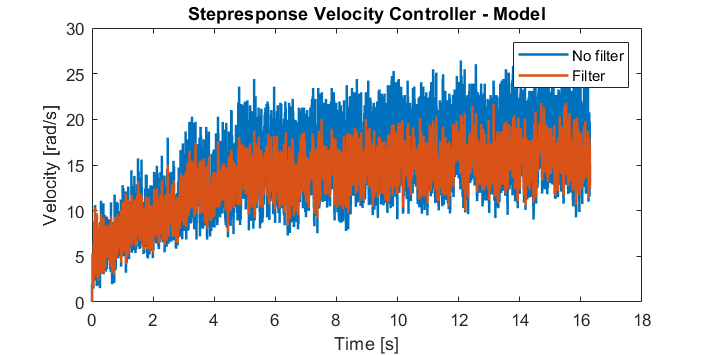
\includegraphics[width=\textwidth]{Sections/Miscellaneous/Images/FilteredStepRespons5Order.png}
    \caption{$5^{th}$ order FIR filter applied to raw velocity feedback data.}
    \label{fig:FilteredStepRespons5Order}
     \end{subfigure}
     \hfill
     \begin{subfigure}[b]{0.49\textwidth}
         \centering
         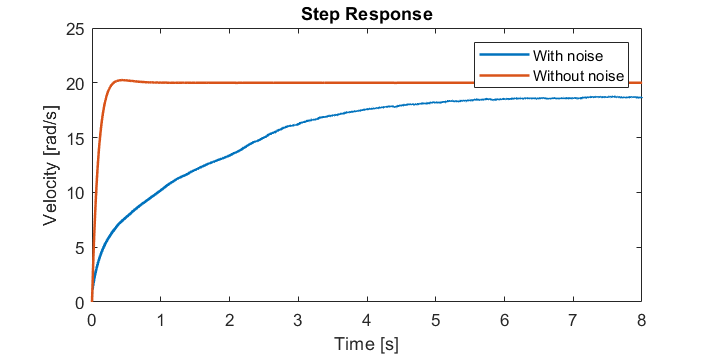
\includegraphics[width=\textwidth]{Sections/Miscellaneous/Images/StepresponsAddedNoise.png}
         \caption{Simulation of the system with added noise.}
         \label{fig:StepResponsAddedNoise}
     \end{subfigure}
        \caption{Simulation results when applying a 5th order FIR to the velocity feedback}
        \label{fig:FilterDiskussionImplementedFilter}
\end{figure}
From figure \ref{fig:StepResponsAddedNoise} it is clear that the noise decreases the rise time and then lowers the value that the response converges towards. On figure \ref{fig:StepResponsAddedNoiseAndFilter} a filter is implemented on the derivative term with transfer function $\frac{5}{1+5/s}$ having a cutoff frequency at $5\,\mathrm{Hz}$. With the noise components at higher frequencies being dampened, it is clear that the derivative term performs much better allowing for faster response and the system almost converging towards the reference at $20\,\frac{\mathrm{rad}}{\mathrm{s}}$. Tilføj noget om hvad filteret betyder ift til vores data, uddyb.\\

\begin{figure}[H]
     \centering
     \begin{subfigure}[b]{0.49\textwidth}
         \centering
    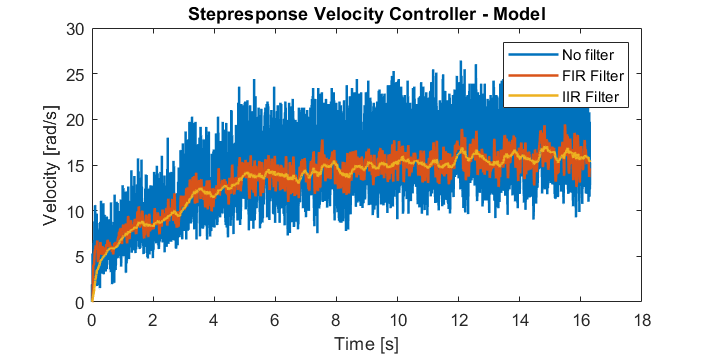
\includegraphics[width=\textwidth]{Sections/Miscellaneous/Images/FilteredStepRespons20Order.png}
    \caption{$20^{th}$ FIR order filter and a first order IIR filter applied to raw velocity feedback data.}
    \label{fig:FilteredStepRespons20Order}
     \end{subfigure}
     \hfill
     \begin{subfigure}[b]{0.49\textwidth}
         \centering
         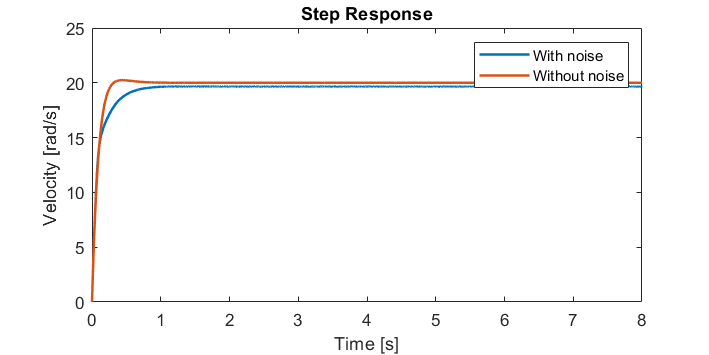
\includegraphics[width=\textwidth]{Sections/Miscellaneous/Images/StepResponsNoiseAndFilter.png}
         \caption{Simulation of the system with added noise and filter on the derivative term.}
         \label{fig:StepResponsAddedNoiseAndFilter}
     \end{subfigure}
        \caption{Simulation results when app}
        \label{fig:FilterDiskussionImplementedFilter20}
\end{figure}
To achieve a response more like in simulation, it would have been favorable to put more time into deliberately designing a filter. On figure \ref{fig:fig:FilteredStepRespons20Order} a $20^{th}$ order filter is applied to the raw velocity feedback data. Even though the amplitude of the data is even smaller than with a $5^{th}$ order filter it is still oscillating. To know if the response would meet the chosen requirements, a test would be necessary. A Infinite Impulse Response (IIR) filter, also displayed on figure \ref{fig:StepResponsAddedNoiseAndFilter}, is another opportunity... Tilføj






\subsection*{Using built-in hardware in the Tiva launchpad}
The project description states that the Basys-3-kit must be used for interfacing with the robot, while the Tiva C-series LaunchPad must handle the user input and that these two development kits must communicate to each other through SPI. However the processing power available on the microcontroller alone or the amount of logic blocks available on the FPGA alone far exceeds the requirements by the scope of the project. Therefore it is possible to implement the project on just one of the platforms. It is clear that the project is constructed in this way to encompass all disciplines, however it is also wanted to clarify that had this project been ordered by an employer it would have been implemented on just one of the platforms. A typical choice could be to implement the system on the microcontroller. The Tiva C-series LaunchPad features peripherals implemented in physical hardware, for handling PWM and getting position and velocity readings from a quadrature encoder. As these are implemented in hardware in the microcontroller and since new data can be flagged by interrupts, eliminating the need for the microcontroller to poll the data, the microcontroller still has plenty of processing power left while handling all the tasks that the FPGA handles right now. The use of the microcontroller as interface to the encoder would also eliminate the delay introduced by the relative slow transmission speed of the SPI connection.      

%\subsection*{Reset from both directions}

\subsection*{Comparison between Simulation and Implementation}
It is noted that it would have beneficial to plot the control signal along with the step responses of all test. This would have made it easier to comprehend and conclude on the behavior of the responses. 
As concluded in the tests section \ref{sec:Test}, there is a difference between the simulated and the implemented response of the controllers. A comparison between the physical step response and the model can be seen on figure \ref{fig:Mes_vs_siml}. The two responses resembles each other fairly well, though if examined further it is seen that there is a difference in the steady state of around 2-3 \si{rad/s}. Also worth noticing is the undulation in the actual response, making it apparent that some parameters are not taken into account or flaws in the estimation of parameters. 

\begin{figure}
    \centering
    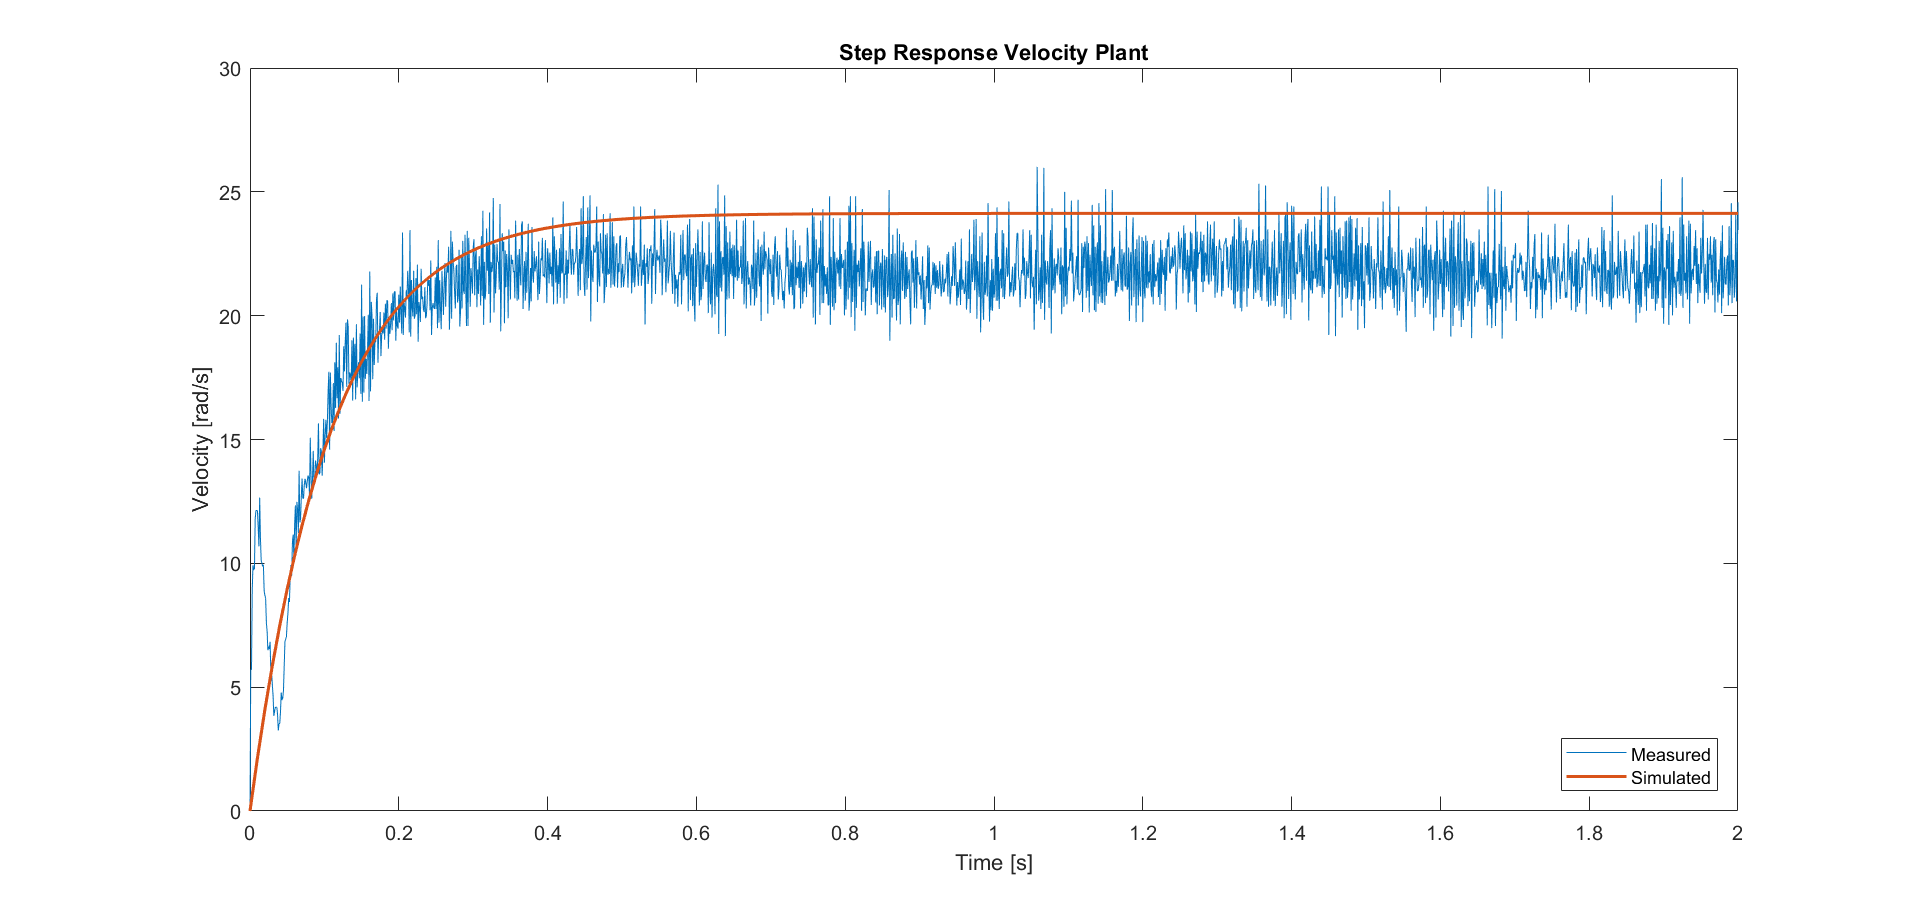
\includegraphics[width = 0.9 \textwidth]{Sections/Miscellaneous/Images/velocityPlantMes_vs_Sim.png}
    \caption{Measured and simulated unrestrained system response}
    \label{fig:Mes_vs_siml}
\end{figure}



\subsection*{Modern Control}
As mentioned in section \ref{sec:Analysis} other control techniques than the PID-controller is available. Modern control techniques uses state feedback to control the system and requires an immense knowledge of the system in question, hence the PID-control was prefered for the project. However it is of great interest to examine the possibility of using modern techniques, enabling the possibility of using observers and estimating otherwise unknown states such as the current. An integral controller with an observer and anti-windup as illustrated on figure \ref{fig:Integral_Observer_Diagram} could be advantageous to implement. The aforementioned constellation introduces four gains to be found namely the feedback gain, $F$, the integral gain, $F_I$, the observer gain, $L$, and anti-windup gain, $M$. The controller leaves a lot of customizability, in the sense that the gains can be tuned to achieve the wanted response of the system, however at the cost of great complexity compared to the PID-controller.


\end{document}